% Auteur\,: Steve Prud’Homme
% Cette oeuvre, création, site ou texte est sous licence Creative Commons Attribution - Pas d’Utilisation Commerciale - Partage dans les Mêmes Conditions 4.0 International. Pour accéder à une copie de cette licence, merci de vous rendre à l'adresse suivante 
% http://creativecommons.org/licenses/by-nc-sa/4.0/ ou envoyez un courrier à 
% Creative Commons, 444 Castro Street, Suite 900, Mountain View, California, 94041, USA.

%::::::::::::::::::::::::::::::::::::::::::::::::::::::::::::::::::::::::::::::::::::::::::::::::::::::::::::::::::::::::::::::::::::::::
%\,:::SNIPET
%::::::::::::::::::::::::::::::::::::::::::::::::::::::::::::::::::::::::::::::::::::::::::::::::::::::::::::::::::::::::::::::::::::::::
%\,::: SECTION
%::::::::::::::::::::::::::::::::::::::::::::::::::::::::::::::::::::::::::::::::::::::::::::::::::::::::::::::::::::::::::::::::::::::::
% \section{Contexte} 
%		\begin{frame}[allowframebreaks]
%			\frametitle{}
%			\begin {itemize}
%				\item 
%			\end{itemize}
%		\end{frame}
%::::::::::::::::::::::::::::::::::::::::::::::::::::::::::::::::::::::::::::::::::::::::::::::::::::::::::::::::::::::::::::::::::::::::
% WATER MARK / FILIGRANE
%::::::::::::::::::::::::::::::::::::::::::::::::::::::::::::::::::::::::::::::::::::::::::::::::::::::::::::::::::::::::::::::::::::::::
%\usepackage{draftwatermark}
%\SetWatermarkLightness{0.5}
%\SetWatermarkAngle{25}
%\SetWatermarkScale{0.5}
%\SetWatermarkFontSize{2cm}
%\SetWatermarkText{Document de travail}
%::::::::::::::::::::::::::::::::::::::::::::::::::::::::::::::::::::::::::::::::::::::::::::::::::::::::::::::::::::::::::::::::::::::::
%PICTURES WITH LINK
%::::::::::::::::::::::::::::::::::::::::::::::::::::::::::::::::::::::::::::::::::::::::::::::::::::::::::::::::::::::::::::::::::::::::
%\begin{figure}
%                     \centering
%                     \includegraphics[width = 0.45\textwidth]{tableau6methodes.png}
%                     \caption{\tiny{\href{run:tableau6methodes.png}{Tableau comparatif des étapes de six méthodes utilisées pour la conception et la réalisation d’outils pédagogiques en ligne \citep[p.20]{bonneau2013a}}}}
%                   \end{figure}
%::::::::::::::::::::::::::::::::::::::::::::::::::::::::::::::::::::::::::::::::::::::::::::::::::::::::::::::::::::::::::::::::::::::::



\documentclass{beamer}
\usepackage{color}
\usepackage{beamerthemesplit} % new 
\usepackage[french]{babel}
\usepackage[utf8]{inputenc}
\usepackage{tikz}
\usepackage[fixlanguage]{babelbib}
\selectbiblanguage{french}
% Natlib pour la bibliographie
\usepackage{natbib}
\usepackage{url}
\usetikzlibrary{mindmap,shadows,shapes,backgrounds}
\usepackage[T1]{fontenc}
\setbeamertemplate{bibliography item}[text]
\usepackage{multicol}


\definecolor{MightySlate}{RGB}{85,98,112}
\definecolor{Pacifica}{RGB}{78,205,196}
\definecolor{AppleChic}{RGB}{199,244,100}
\definecolor{CheeryPink}{RGB}{255,107,107}

\setbeamercolor{titlelike}{parent=structure}
\setbeamerfont*{title}{size=\huge}
\setbeamercolor{title}{bg=MightySlate, fg=white}
\setbeamercolor{author}{bg=Pacifica, fg=white}
\setbeamercolor{institute}{bg=AppleChic, fg=black}
\setbeamercolor{date}{bg=CheeryPink, fg=white}

\definecolor{DTUred}{RGB}{178,20,20}
\setbeamercolor*{palette primary}{use=structure,fg=white,bg=MightySlate}
\usepackage{helvet}
%\usepackage{draftwatermark}
%\SetWatermarkLightness{0.5}
%\SetWatermarkAngle{25}
%\SetWatermarkScale{0.5}
%\SetWatermarkFontSize{2cm}
%\SetWatermarkText{Document de travail}

\begin{document}
	\title{Réaliser rapidement et facilement des animations PRO} 
	\author{Steve Prud'Homme} 
	\institute{Commission scolaire de Laval} 
	\date{\today} 

	
	\usebackgroundtemplate{%
  \includegraphics[height=\paperheight]{back.jpg}} 
	
	\begin{frame}
	\end{frame}
	\frame{\titlepage} 
	
	\usebackgroundtemplate{ } 
	\par L’intention de ce document est de respecter pleinement les droits des créateurs des ressources
utilisées.
	\par En ce qui concerne les citations insérées selon le principe de l'utilisation équitable ou avec la permission de l'auteur, veuillez les contacter ou respecter les droits d’utilisation précisés dans les documents d’origine avant de les réutiliser.
	\par Si vous estimez que certains éléments de ce document ne respectent pas intégralement les droits de vos
publications, veuillez nous en aviser afin que les modifications nécessaires puissent être apportées au\,: \url{mailto:sprudhomme@cslaval.qc.ca}.
	\par Cette \oe uvre, création, site ou texte est sous licence Creative Commons Attribution\,-\,Pas d’Utilisation Commerciale\,-\,Partage dans les Mêmes Conditions 4.0 International.
	\section{Sommaire} 
		\begin{frame}
			Cette présentation vise à\,:
			\frametitle{Sommaire}
			\begin {itemize}
				\item \textbf{Bref aperçu des outils} 
				\item Pertinence des \textbf{pratiques harmonisées}.
				\item Pertinence d'avoir \textbf{un esprit critique en ce qui concerne les modèles d'affaire des outils utilisés}.

			\end{itemize}
		\end{frame}
	\frame[allowframebreaks]{\frametitle{Ordre du jour}\tableofcontents}

\section{La réalisation de séquences vidéo animées} 
		
	
\subsection{Qui ?} 
		\begin{frame}[allowframebreaks]
			\frametitle{Qui est-ce qui utilise les séquences vidéo ?}
			\begin {itemize}
				\item Responsable du marketeing
				\item Les formateurs
				\item Les communicateurs

			\end{itemize}
		\end{frame}

\subsection{Enjeux} 
		\begin{frame}[allowframebreaks]
		 \frametitle{Enjeux lors de réalisation de séquence vidéo d'animation}
			\begin{figure}
                   
                      \centering
                     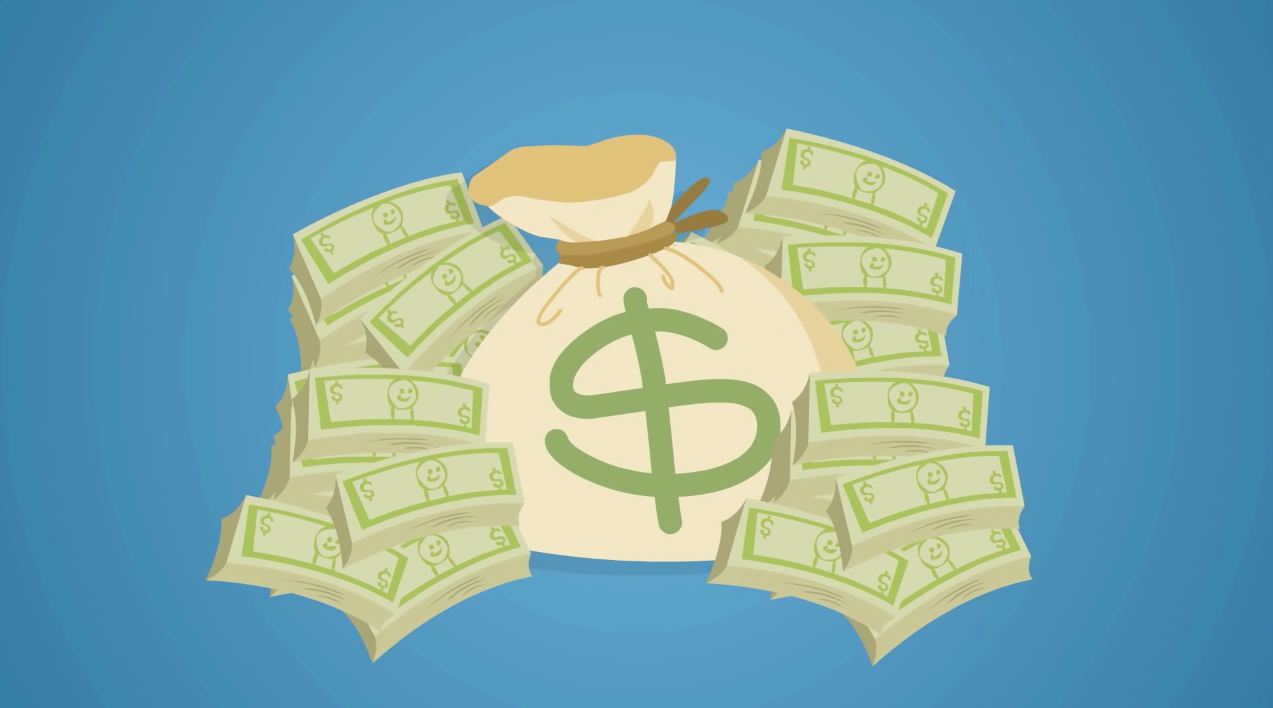
\includegraphics[width = 0.5\textwidth]{cout.png}
                     \caption{\tiny{\href{run:cout.png}{Le coût.}}}
                   \end{figure}
			
			
			
			
			\begin{description}[Second Item]
				\item[Coût] De 1000 \$ à 10 0000 \$.
			\end{description}
			\framebreak
			
			\begin{figure}
                     \centering
                     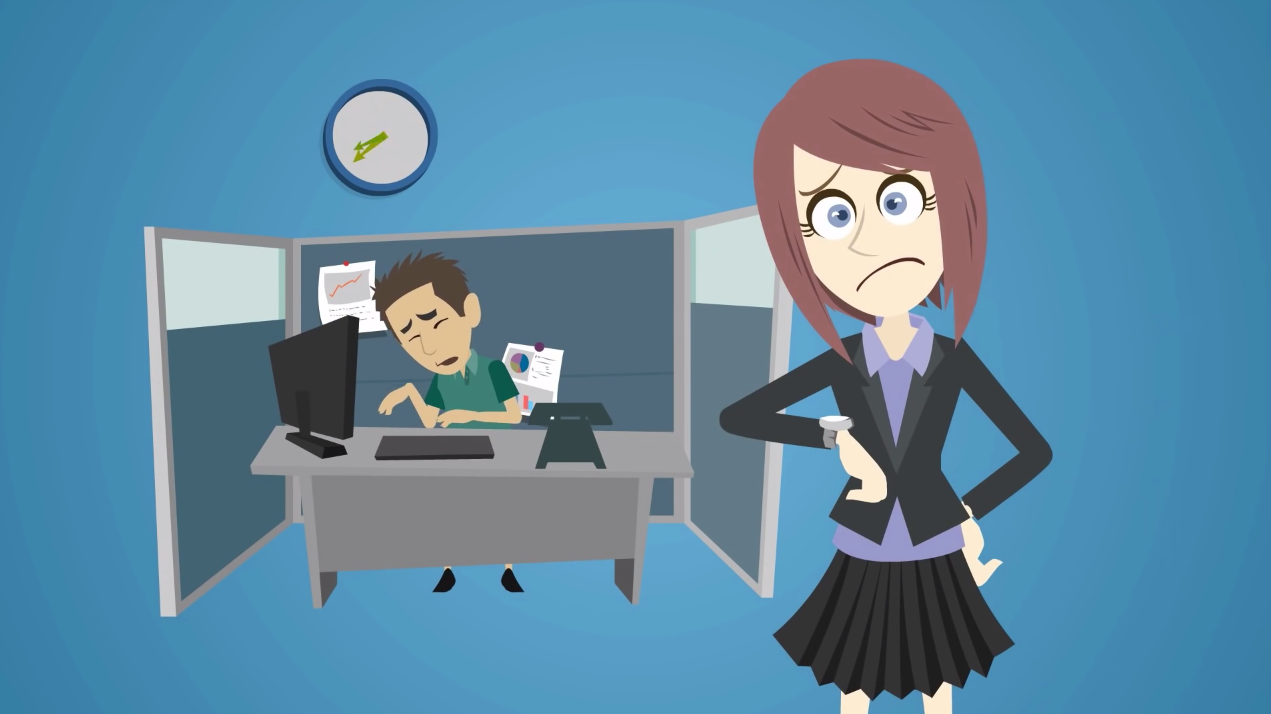
\includegraphics[width = 0.5\textwidth]{temps.png}
                     \caption{\tiny{\href{run:temps.png}{Le temps.}}}
                   \end{figure}
			
			
			\begin{description}[Second Item]
				\item[Temps] Production et postproduction peut prendre des semaines ou même des mois.
				
			\end{description}
			\framebreak
			
			\begin{figure}
                     \centering
                     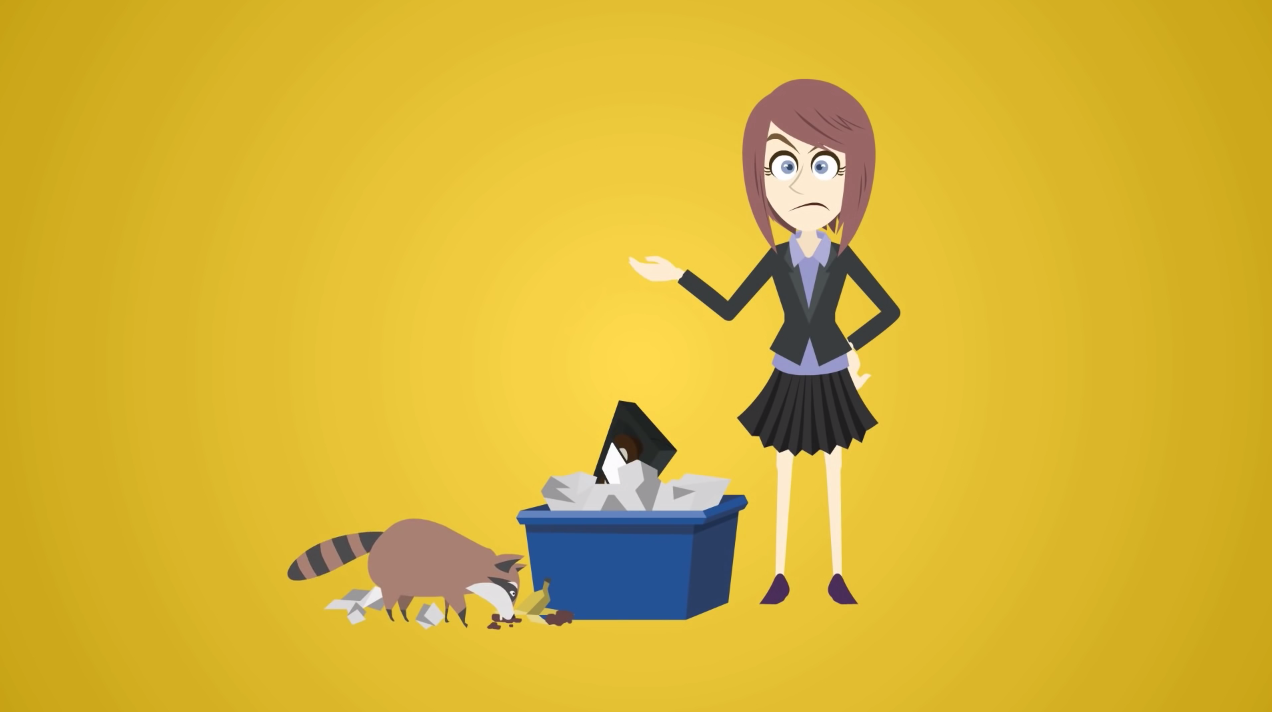
\includegraphics[width = 0.5\textwidth]{risque.png}
                     \caption{\tiny{\href{run:risque.png}{Le risque.}}}
                   \end{figure}
			
			\begin{description}[Second Item]
				\item[Risques] On peut couler le budget ou même finir avec un produit qu'il est impossible d'utiliser.
				
			\end{description}
				
		\end{frame}
\subsection{Bidouiller (DIY)} 
		\begin{frame}[allowframebreaks]
			\frametitle{Bidouiller une séquence vidéo animée (\textit{do-it yourself})}
			\begin{figure}
                     \centering
                     \includegraphics[width = 0.5\textwidth]{crazytalk.jpg}
                     \caption{\tiny{\href{run:crazytalk.jpg}{Capture d'écran du logiciel Crazy Talk Animator 2 \citep{ReallusionInc2016}}}}
                   \end{figure}
			\framebreak
			\begin{figure}
                     \centering
                     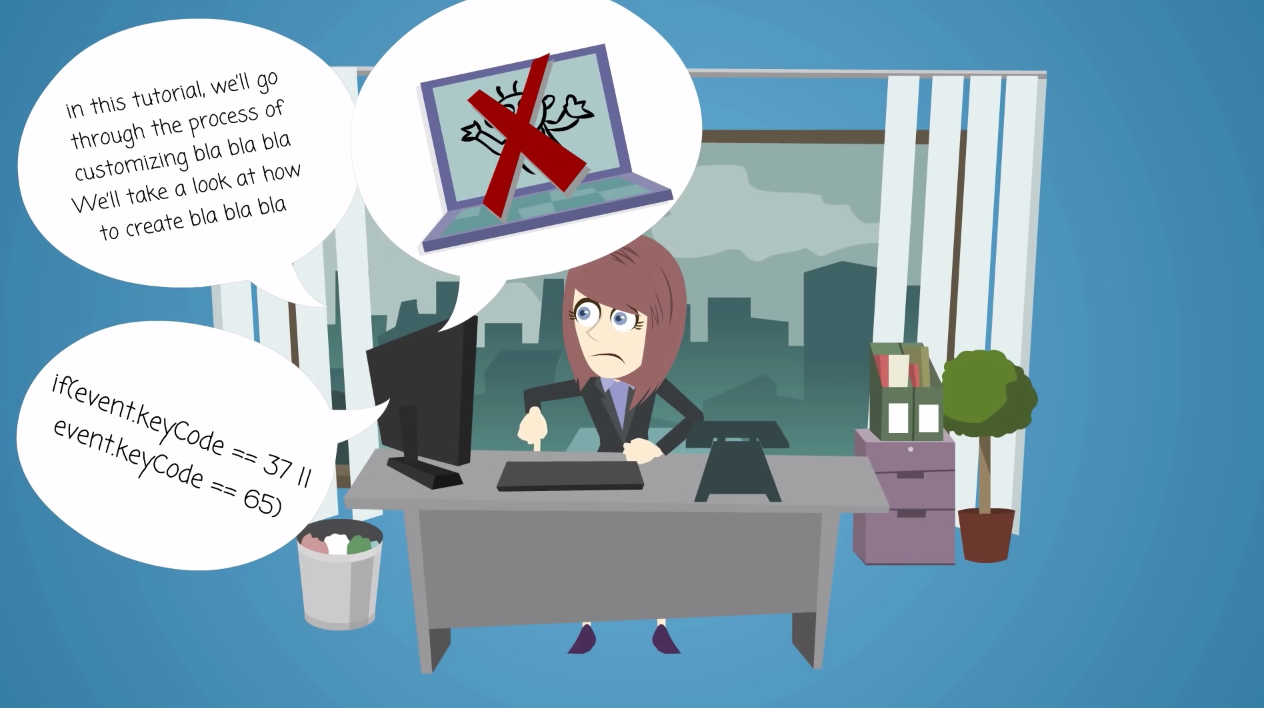
\includegraphics[width = 0.5\textwidth]{apprentissage.png}
                     \caption{\tiny{\href{run:apprentissage.png}{Apprentissage difficile.}}}
                   \end{figure}
			\begin {itemize}
				\item Les logiciels sur PC / Mac sont difficilles.
				\item La courbe d'apprentissage est grande.

			\end{itemize}
			\end{frame}	
			

\section{GoAnimate} 

\subsection{Quoi ?} 
		\begin{frame}
			\frametitle{Qu'est-ce que GoAnimate ?}
			\begin{figure}
                     \centering
                     
\includegraphics[width = 0.6\textwidth]{goanimate.png}
                     \caption{\tiny{\href{run:goanimate.png}{Le logiciel GoAnimate.}}}
                   \end{figure}
			Site internet où il est possible de réaliser rapidement et facilement des séquences vidéo animées professionelles.
			\end{frame}	
			
\subsection{Pour faire quoi ?} 
		\begin{frame}[allowframebreaks]
			\frametitle{Qu'est-ce que je peux faire avec GoAnimate ?}
			\begin{figure}
                     \centering
                     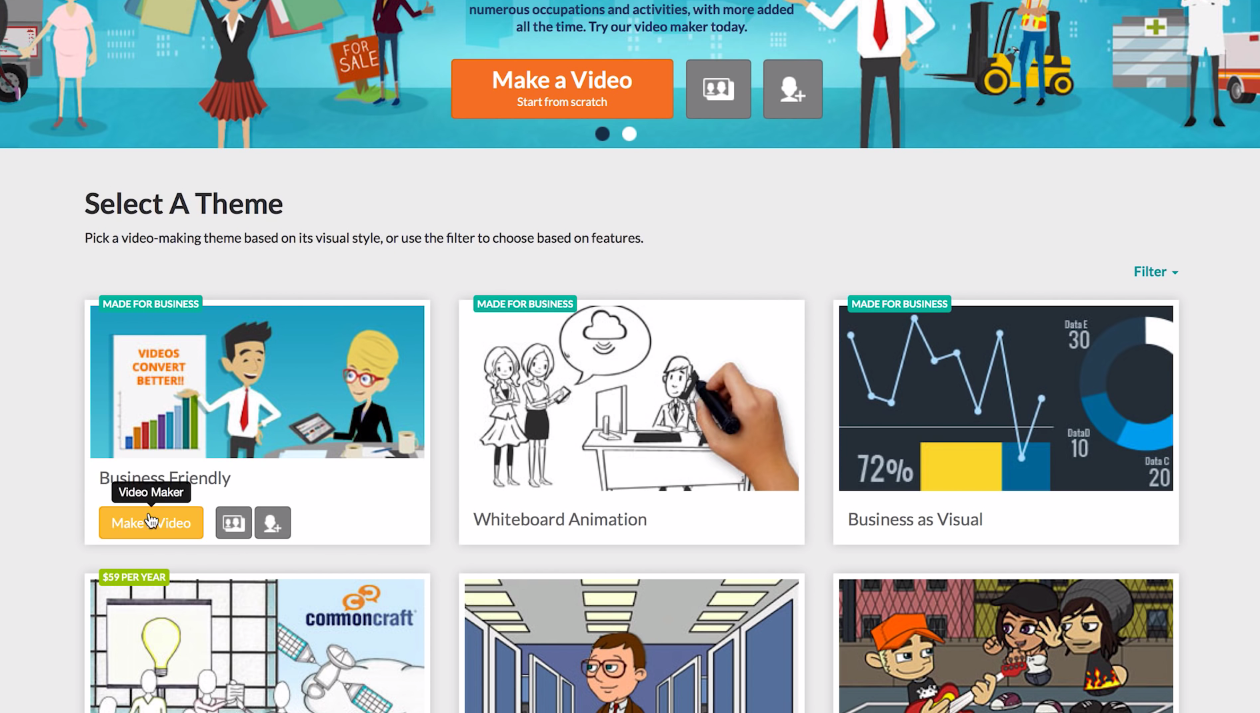
\includegraphics[width = 0.7\textwidth]{theme.png}
                     \caption{\tiny{\href{run:theme.png}{Choisir un thème créatif en 1 clique.}}}
                   \end{figure}
                   
                   \begin{figure}
                     \centering
                     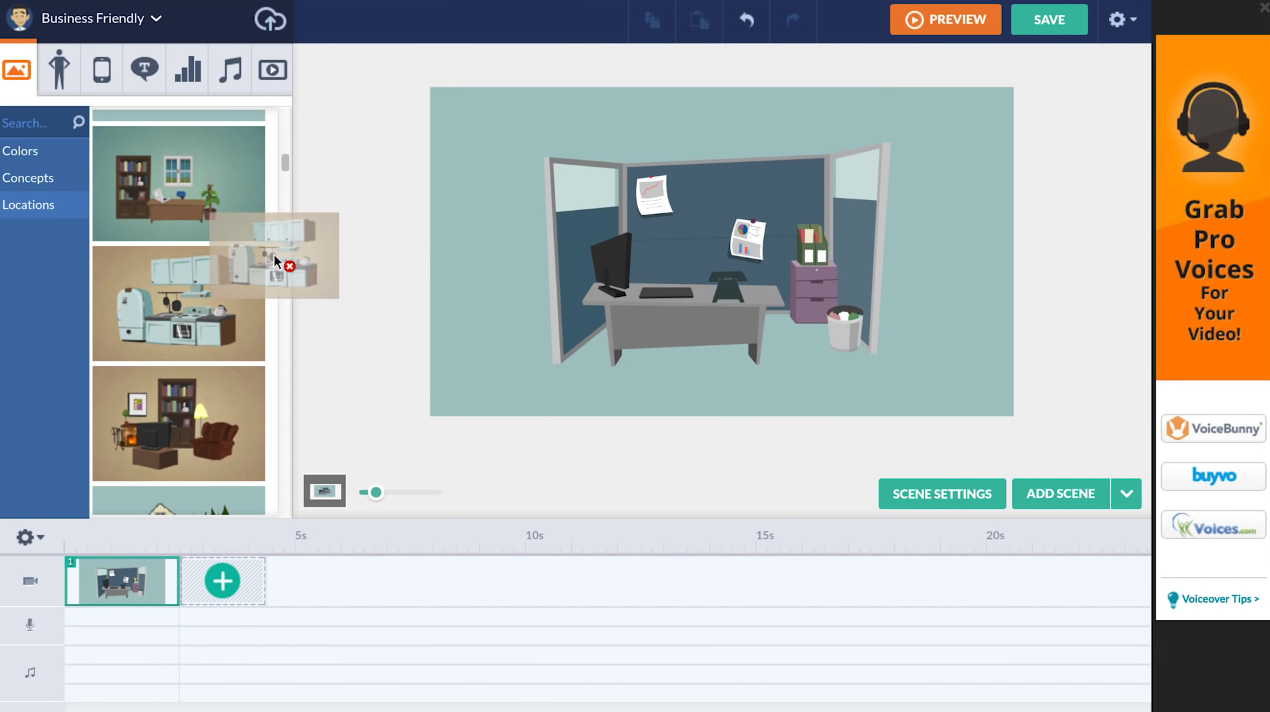
\includegraphics[width = 0.7\textwidth]{decors.png}
                     \caption{\tiny{\href{run:decors.png}{Choisir un arrière plan (décor) en effectuant un glisser-déposer.}}}
                   \end{figure}
                   
                   \begin{figure}
                     \centering
                     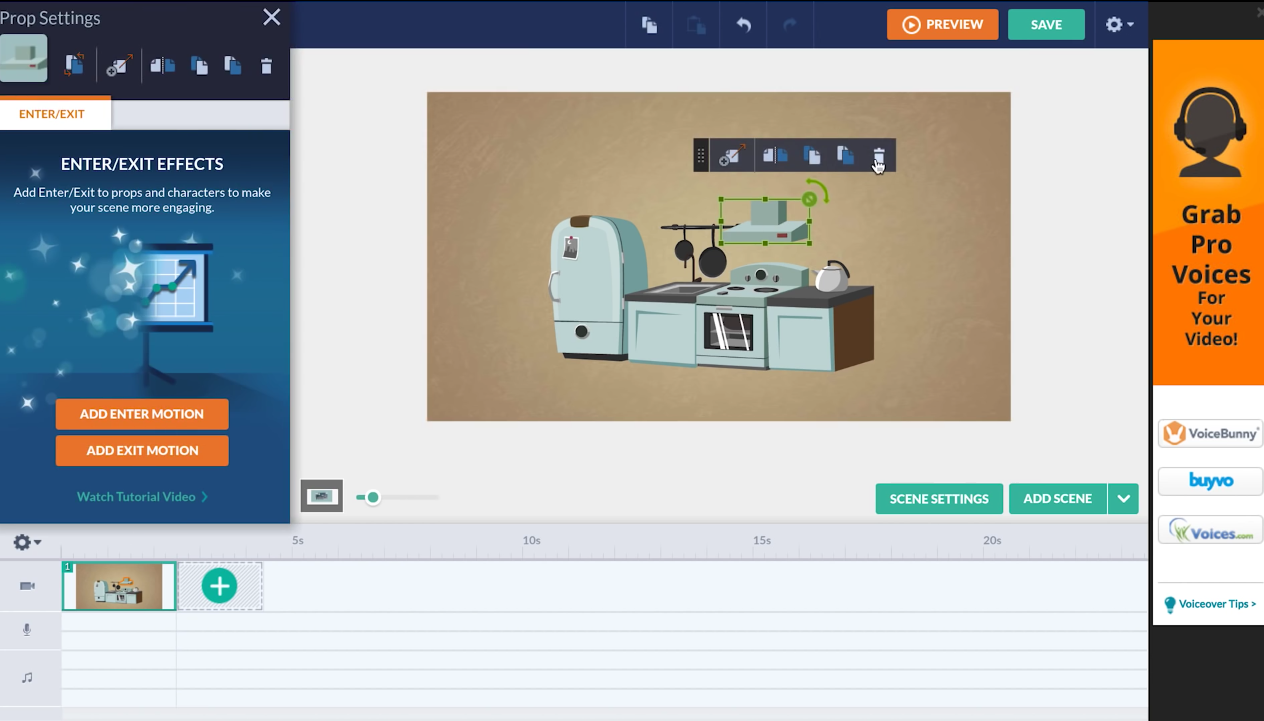
\includegraphics[width = 0.7\textwidth]{modifierdecor.png}
                     \caption{\tiny{\href{run:modifierdecor.png}{Modifier l'arrière-plan (décor) en quelques cliques.}}}
                   \end{figure}
                   
                   \begin{figure}
                     \centering
                     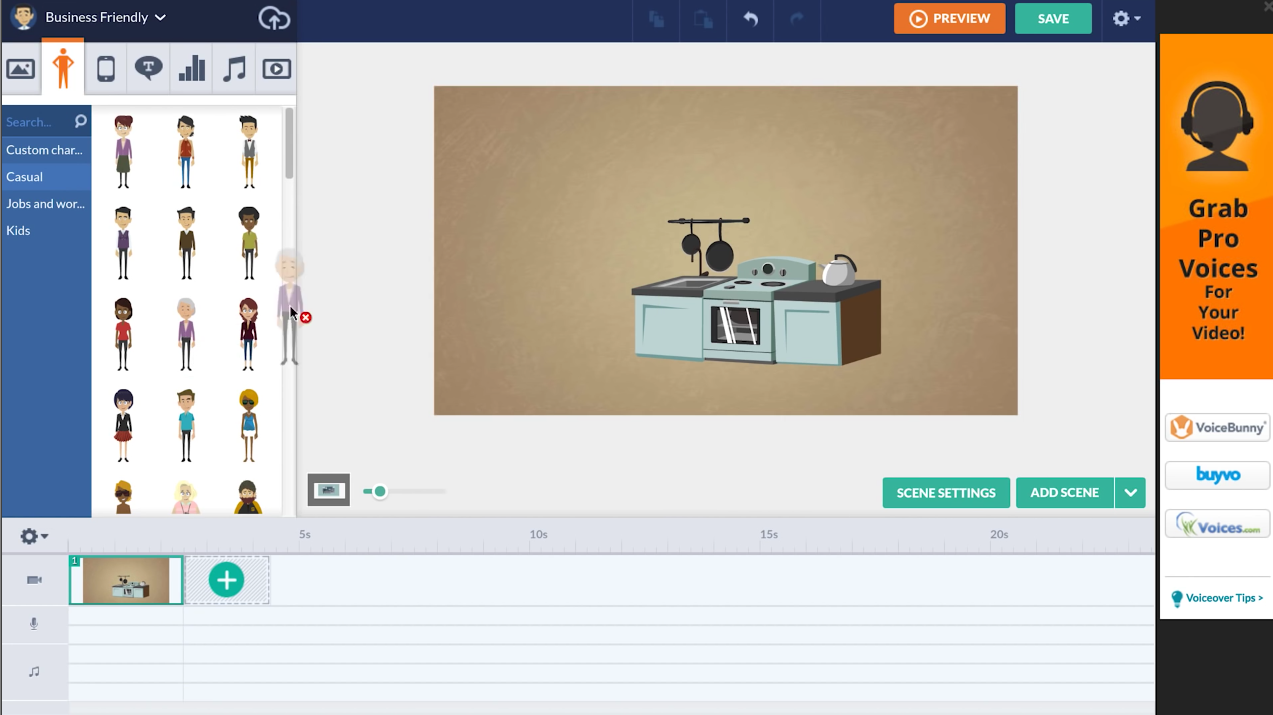
\includegraphics[width = 0.7\textwidth]{personnage.png}
                     \caption{\tiny{\href{run:personnage.png}{Ajouter et modifier facielement des caractères. Attribuer aisément des actions aux caractères.}}}
                   \end{figure}
                   
                    \begin{figure}
                     \centering
                     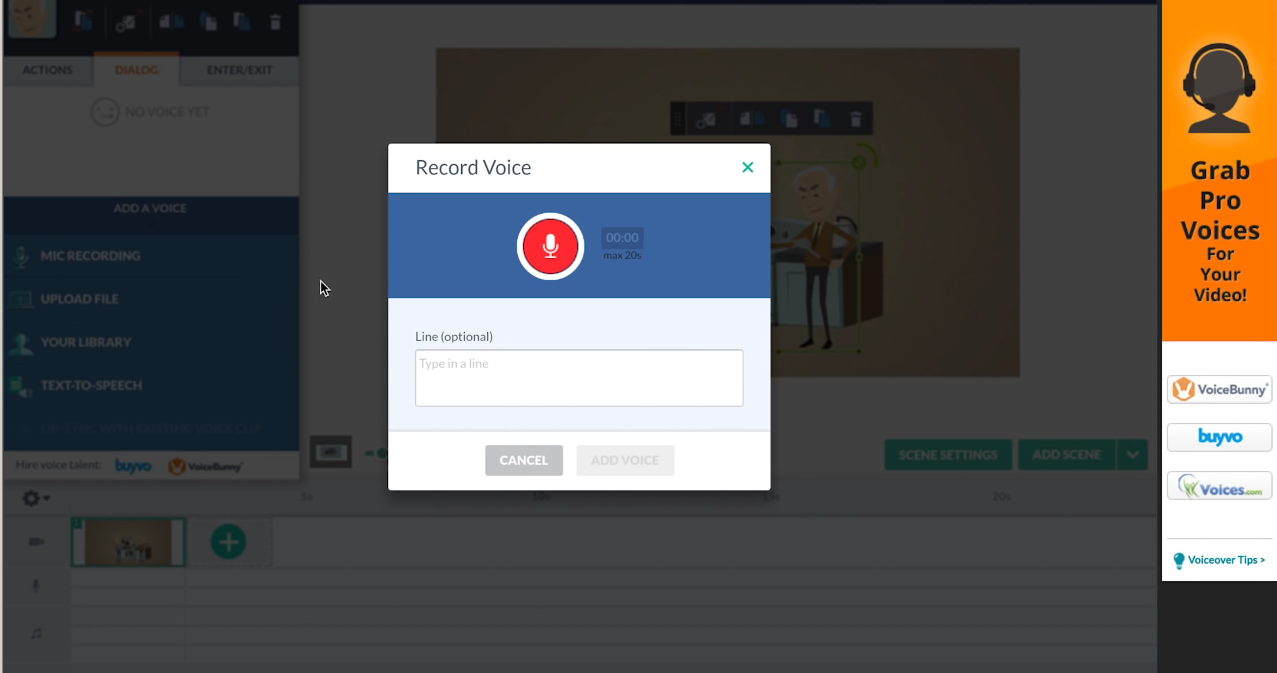
\includegraphics[width = 0.7\textwidth]{voix.png}
                     \caption{\tiny{\href{run:voix.png}{Enregistrer un dialogue ou engager un comédien.}}}
                   \end{figure}
                   
                   \begin{figure}
                     \centering
                     
\includegraphics[width = 0.7\textwidth]{autres.png}
                     \caption{\tiny{\href{run:autres.png}{Utiliser des séquences modèles, séquences (props), entrée et sortie de scène, musique, effets sonores, etc.}}}
                   \end{figure}
                   
			
			
			\end{frame}	
\subsection{Modèle d'affaire} 
		\begin{frame}[allowframebreaks]
			\frametitle{Le modèle d'affaire de GoAnimate}
			\begin{figure}
			\centering
                     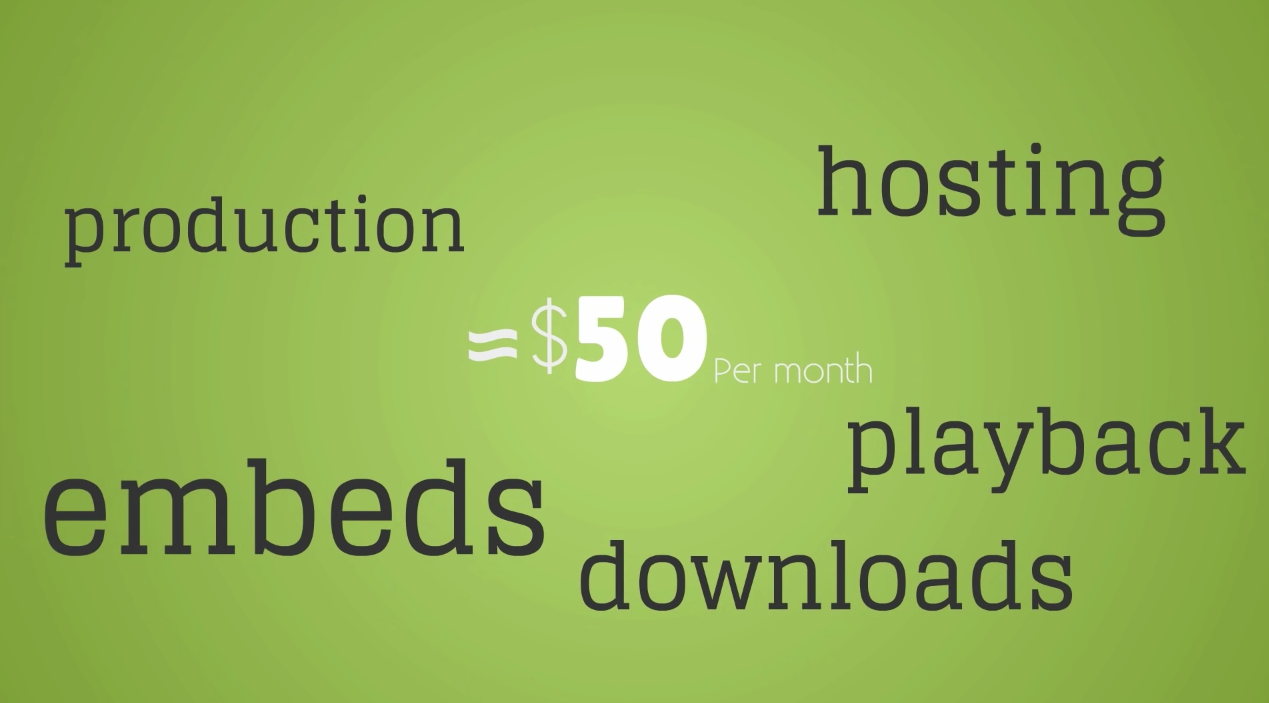
\includegraphics[width = 0.7\textwidth]{modeleaffaire.png}
                     \caption{\tiny{\href{run:modeleaffaire.png}{Le modèle d'affaire de GoAnimate.}}}
                   \end{figure}
			\framebreak
			\begin {itemize}
				\item 50 \$ US par mois.
				\item Productions illimités
				\item Hébergement illimité
				\item Visionnements illimités
				\item Encapsulations illimités
				\item Téléchargements illimités
				\item Exports illimités vers des aggragateurs comme YouTube, Hubspot, Lectora Online, etc.

			\end{itemize}
			
			\end{frame}	
			
\section{Nawmal} 
\subsection{Quoi ?} 
		\begin{frame}
			\frametitle{Qu'est-ce que Nawmal ?}
			\begin{figure}
                     \centering
                     
\includegraphics[width = 0.6\textwidth]{goanimate.png}
                     \caption{\tiny{\href{run:goanimate.png}{Le logiciel GoAnimate.}}}
                   \end{figure}
			Logiciel hybride avec lequel  il est possible de réaliser rapidement et facilement des séquences vidéo animées 3d professionelles.
			\end{frame}		
\subsection{Pour faire quoi ?} 
		\begin{frame}[allowframebreaks]
			\frametitle{Qu'est-ce que je peux faire avec Nawmal ?}
			\begin{figure}
                     \centering
                     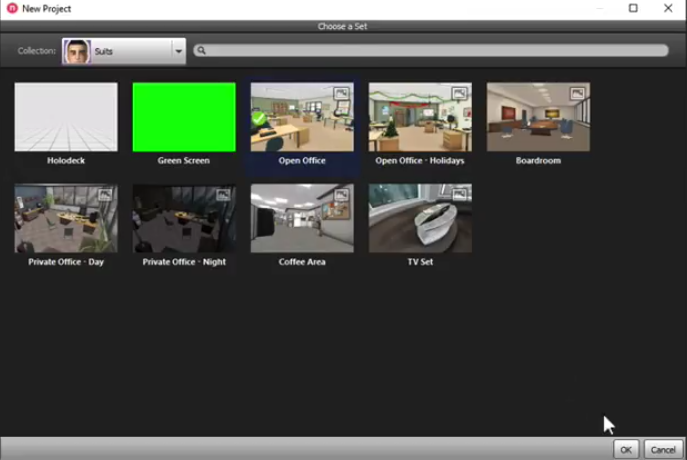
\includegraphics[width = 0.6\textwidth]{nawmaldecor2.png}
                     \caption{\tiny{\href{run:nawmaldecor.2png}{Choisir un décors créatif en 1 clique.}}}
                   \end{figure}
                   
                   \begin{figure}
                     \centering
                     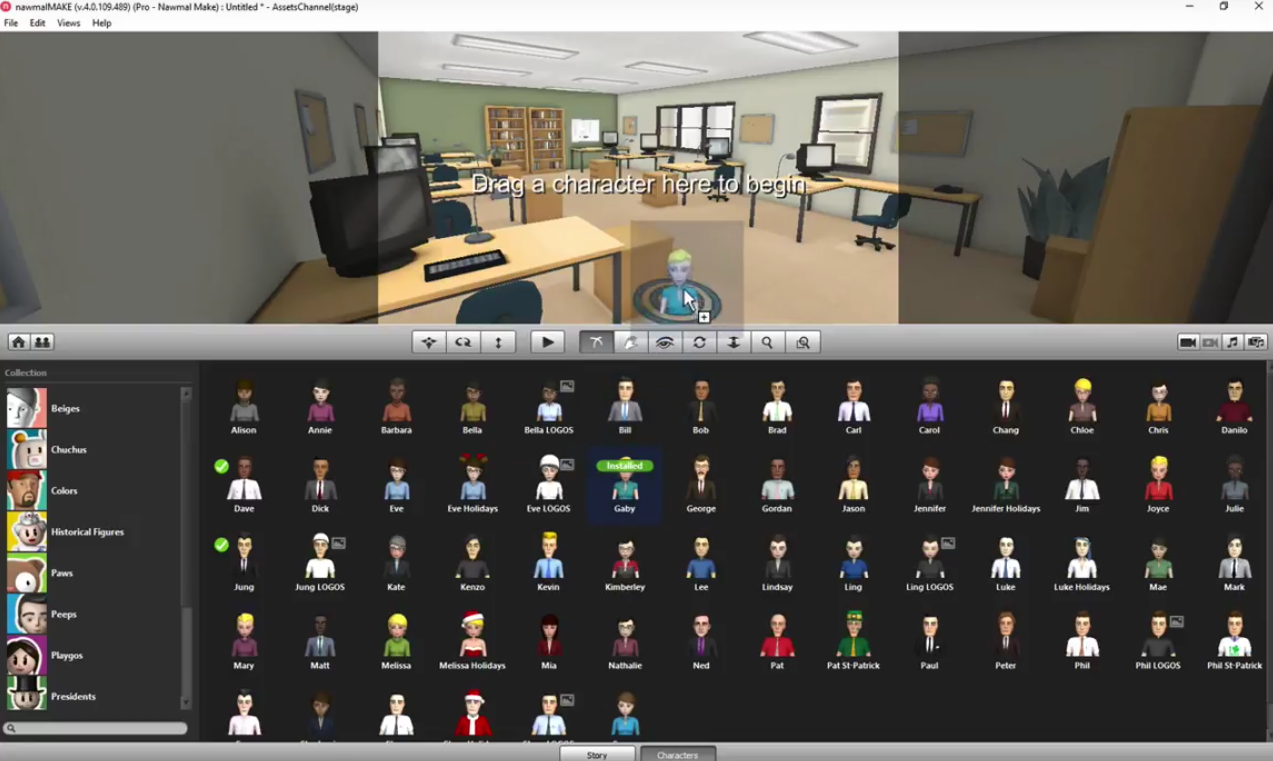
\includegraphics[width = 0.6\textwidth]{nawmalpersonnage2.png}
                     \caption{\tiny{\href{run:nawmalpersonnage2.png}{Choisir un personnage.}}}
                   \end{figure}
                   
                   \begin{figure}
                     \centering
                     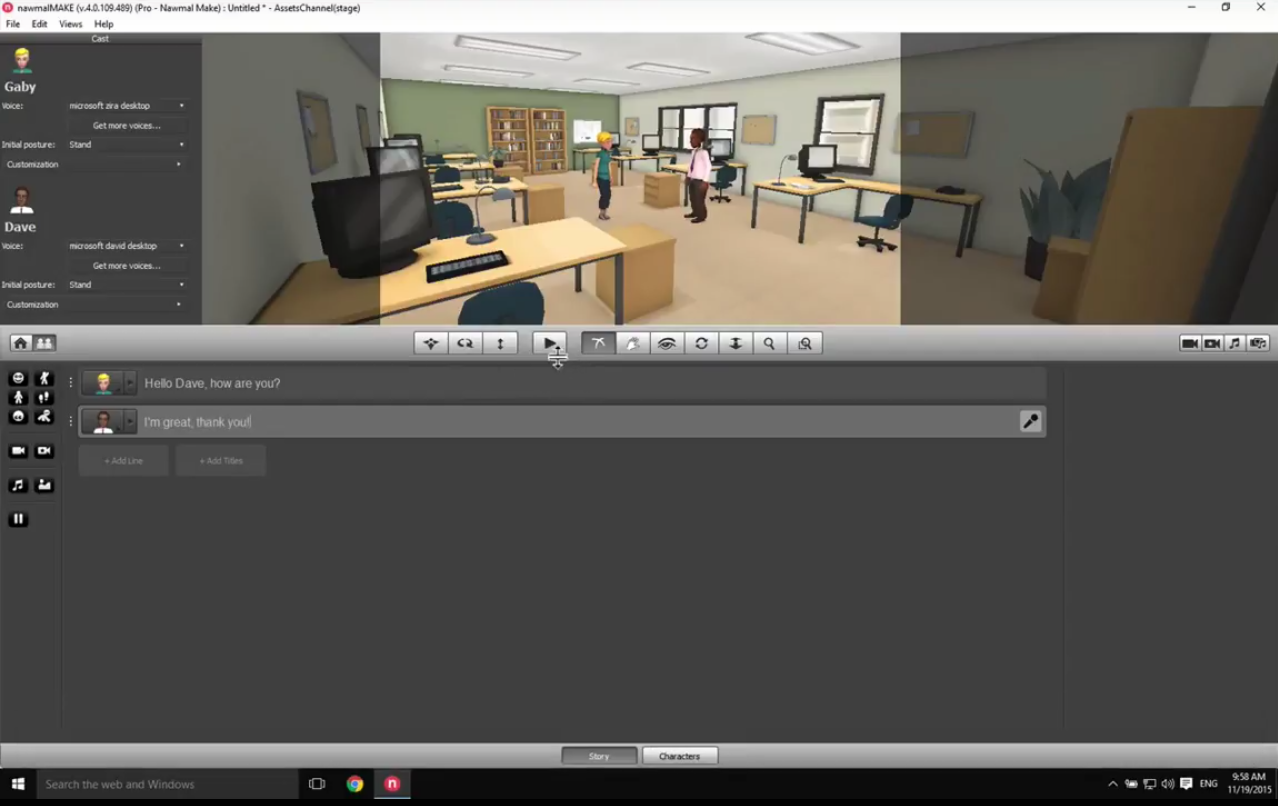
\includegraphics[width = 0.6\textwidth]{nawmaldialogue2.png}
                     \caption{\tiny{\href{run:nawmaldialogue2.png}{Écrire le dialogue}}}
                   \end{figure}
                   
                   								
			\end{frame}	
			
																														\subsection{Fexibilité} 
		\begin{frame}[allowframebreaks]
			\frametitle{La flexibilité de Nawmal}
			\begin{figure}
			\centering
                     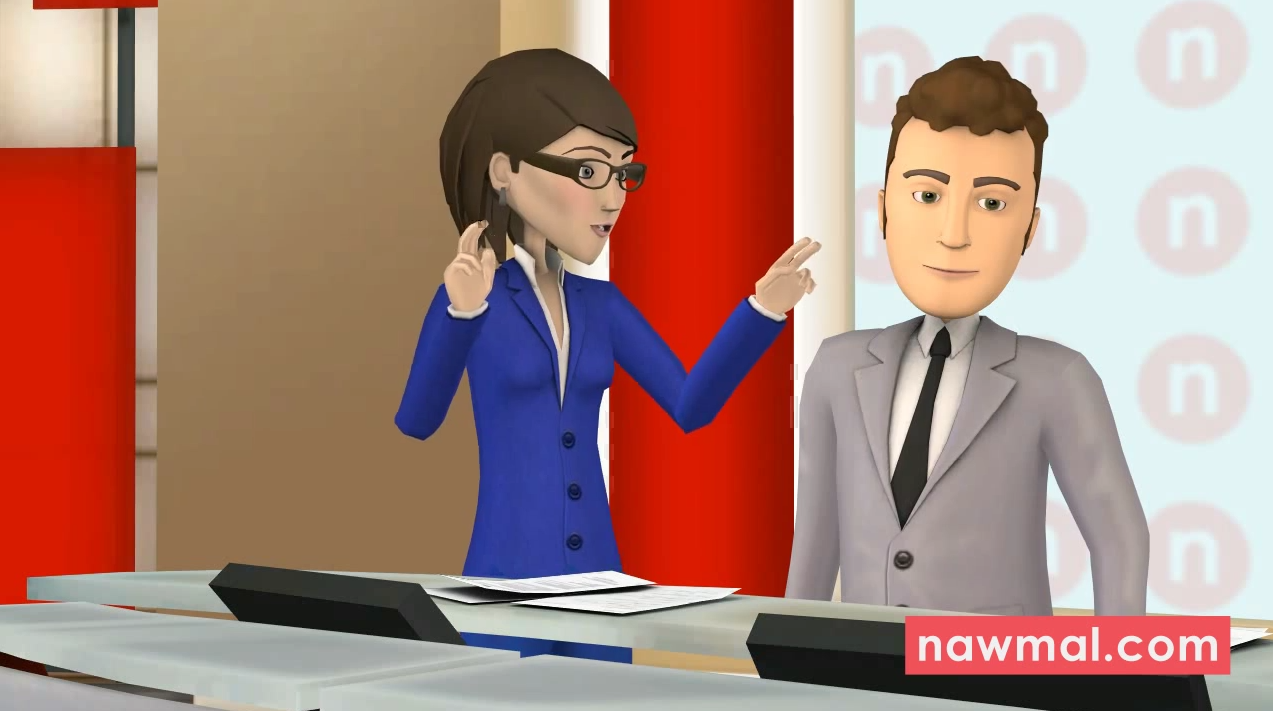
\includegraphics[width = 0.8\textwidth]{nawmalflexibilite.png}
                     \caption{\tiny{\href{run:nawmalflexibilite.png}{La fexibilité de Nawmal}}}
                   \end{figure}
			\framebreak
			\begin {itemize}
				\item Choisir parmis 100 gestuels
				\item Faire marcher le personnage
				\item Contrôler les angles et mouvements de la caméra
				\item Ajouter un titre, de la musique et des effets sonores.
				

			\end{itemize}
			
			\end{frame}	
			
																														\subsection{Modèle d'affaire} 
		\begin{frame}[allowframebreaks]
			\frametitle{Le modèle d'affaire de Nawmal}
			\begin{figure}
			\centering
                     
\includegraphics[width = 1\textwidth]{nawmalmodeleaffaire.png}
                     \caption{\tiny{\href{run:nawmalmodeleaffaire.png}{Le modèle d'affaire de Nawmal}}}
                   \end{figure}
		
			\end{frame}		
			
\section{Critique et autres outils} 
\subsection{Critique de ces nouveaux produit} 
		\begin{frame}[allowframebreaks]
			\frametitle{Critique de ces nouveaux produit}
			\begin{figure}
			\centering
                     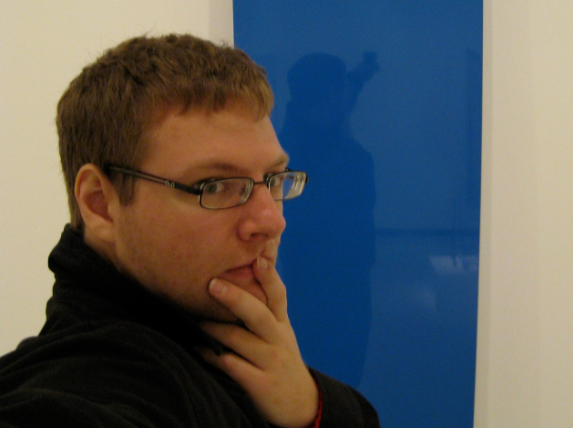
\includegraphics[width = 0.6\textwidth]{critique.png}
                     \caption{\tiny{\href{run:critique.png}{Critique. Photographie de \citet{Mosler2007} CC-BY-SA}}}
                   \end{figure}
			\framebreak
			\begin {itemize}
				\item Modèle d'affaire web ou hybride basé sur l'abonnement.
				\item Le client est tributaire du fournisseur
				\item Impossibilité d'avoir accès au fichier source.
				\item La périnité et l'interopérabilité d'un tel produit ne peu pas être assuré.
				

			\end{itemize}																											\end{frame}		
			
\subsection{Autre outil : iClone} 
		\begin{frame}[allowframebreaks]
			\frametitle{Critique de ces nouveaux produit}
			
			\begin{figure}
			\centering
                     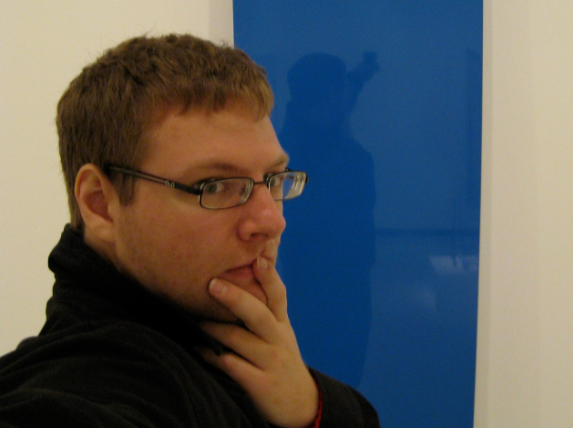
\includegraphics[width = 0.6\textwidth]{critique.png}
                     \caption{\tiny{\href{run:critique.png}{Critique. Photographie de \citet{Mosler2007} CC-BY-SA}}}
                   \end{figure}
			\framebreak
																														\end{frame}		
																												
%\section{Bibliographie}
%\subsection{Bibliographie}
\frame[allowframebreaks]{\frametitle{Bibliographie}

\bibliographystyle{apalike}
\bibliography{bibliographie} %bibtex file name without .bib extension
}
\framebreak
\par L’intention de ce document est de respecter pleinement les droits des créateurs des ressources
utilisées.
	\par En ce qui concerne les citations insérées selon le principe de l'utilisation équitable, veuillez les contacter ou respecter les droits d’utilisation précisés dans les documents d’origine avant de les réutiliser.
	\par Si vous estimez que certains éléments de ce document ne respectent pas intégralement les droits de vos
publications, veuillez nous en aviser afin que les modifications nécessaires puissent être apportées au\,: \url{mailto:sprudhomme@cslaval.qc.ca}.
	\par Cette \oe uvre, création, site ou texte est sous licence Creative Commons Attribution\,-\,Pas d’Utilisation Commerciale\,-\,Partage dans les Mêmes Conditions 4.0 International. \\
	\par 
	 Pour accéder à une copie de cette licence, merci de vous rendre à l'adresse suivante\,: \url{http://creativecommons.org/licenses/by-nc-sa/4.0/} ou envoyez un courrier à 

\par Creative Commons, 444 Castro Street, Suite 900, Mountain View, California, 94041, USA.
\par Ce document a été réalisé en \LaTeX, avec l'environnement Beamer. Vous pouvez trouver le code source ici\,: \url{https://goo.gl/BRB6pM}. Vous pouvez avoir accès à cette présentation ainsi qu'à d'autres ressources sur\url {https://goo.gl/jvzi0s}
\end{document}

